\documentclass[20pt,a0paper,landscape,
  margin=0mm,innermargin=12mm,
  blockverticalspace=10mm,
  colspace=12mm,subcolspace=6mm]{tikzposter}

% Shrink the page height to ~16:9 so content fills.
% Keep tikzposter's a0paper-landscape width (1189mm) so its column
% layout is unchanged; just trim the unused vertical space.
\setlength{\pdfpageheight}{669mm}
\setlength{\paperheight}{669mm}

\usepackage[utf8]{inputenc}
\usepackage[T1]{fontenc}
\usepackage{lmodern}
\renewcommand{\familydefault}{\sfdefault}
\usepackage{amsmath,amssymb,booktabs}
\usepackage{tikz}
\usepackage{pgfplots}
\usepackage{xcolor}
\pgfplotsset{compat=1.18}
\usetikzlibrary{arrows.meta,positioning,calc,shadows}

\usetheme{Default}

\definecolor{posterNavy}{RGB}{15,35,80}
\definecolor{posterMagenta}{RGB}{210,25,110}
\definecolor{posterTeal}{RGB}{0,140,140}
\definecolor{posterTealLight}{RGB}{225,245,243}
\definecolor{posterGrey}{RGB}{245,245,245}
\definecolor{posterGreen}{RGB}{0,120,110}
\definecolor{posterOrange}{RGB}{230,130,30}
\definecolor{posterAccent}{RGB}{255,170,60}
\definecolor{posterBgTop}{RGB}{248,250,253}
\definecolor{posterBgBot}{RGB}{236,240,247}

\definecolorpalette{NavyMagenta}{%
  \definecolor{colorOne}{named}{posterNavy}%
  \definecolor{colorTwo}{named}{posterMagenta}%
  \definecolor{colorThree}{named}{posterGrey}%
}
\usecolorpalette{NavyMagenta}

\colorlet{backgroundcolor}{posterBgTop}
\colorlet{framecolor}{posterNavy}
\colorlet{titlebgcolor}{posterNavy}
\colorlet{titlefgcolor}{white}
\colorlet{blocktitlebgcolor}{posterMagenta}
\colorlet{blocktitlefgcolor}{white}
\colorlet{blockbodybgcolor}{white}
\colorlet{blockbodyfgcolor}{black}

% --- soft gradient background ---
\definebackgroundstyle{StylishBg}{
  \draw[inner sep=0pt,outer sep=0pt,top color=posterBgTop,bottom color=posterBgBot]
    (bottomleft) rectangle (topright);
}
\usebackgroundstyle{StylishBg}

% --- bold title bar with gradient + accent stripes ---
\definetitlestyle{StylishTitle}{
  width=\paperwidth, roundedcorners=0, linewidth=0pt,
  innersep=26pt, titletotopverticalspace=0mm,
  titletoblockverticalspace=14mm,
  titlegraphictotitledistance=0pt
}{
  % deep navy → midnight gradient
  \shade[top color=posterNavy!92,bottom color=posterNavy]
    (\titleposleft,\titleposbottom) rectangle (\titleposright,\titlepostop);
  % subtle decorative diagonal lines on the right
  \begin{scope}
    \clip (\titleposleft,\titleposbottom) rectangle (\titleposright,\titlepostop);
    \foreach \i in {0,...,40}{
      \draw[white,opacity=0.04,line width=1pt]
        ($(\titleposright,\titlepostop)+(-\i*30pt,0)$) --
        ($(\titleposright,\titleposbottom)+(-\i*30pt-180pt,0)$);
    }
  \end{scope}
  % bottom accent: thick magenta + thin amber
  \fill[posterMagenta] (\titleposleft,\titleposbottom) rectangle (\titleposright,\titleposbottom+11pt);
  \fill[posterAccent]  (\titleposleft,\titleposbottom+11pt) rectangle (\titleposright,\titleposbottom+15pt);
  % top hairline
  \fill[posterMagenta!70] (\titleposleft,\titlepostop-3pt) rectangle (\titleposright,\titlepostop);
}
\usetitlestyle{StylishTitle}

% --- rounded block with soft drop shadow & accent rule under title ---
\defineblockstyle{Stylish}{
  titlewidthscale=1, bodywidthscale=1, titlecenter,
  titleoffsetx=0pt, titleoffsety=0pt,
  bodyoffsetx=0pt, bodyoffsety=0pt,
  bodyverticalshift=0pt,
  roundedcorners=14, linewidth=0.7pt,
  titleinnersep=11pt, bodyinnersep=14pt
}{
  \draw[draw=posterNavy!18,line width=0.7pt,fill=blockbodybgcolor,
        rounded corners=\blockroundedcorners,
        drop shadow={shadow xshift=0pt,shadow yshift=-3pt,opacity=0.18,fill=posterNavy}]
    (blockbody.south west) rectangle (blockbody.north east);
  \ifBlockHasTitle
    \draw[draw=none,fill=blocktitlebgcolor,rounded corners=\blockroundedcorners]
      (blocktitle.south west) rectangle (blocktitle.north east);
    % square the bottom edge so title sits flush on body
    \fill[blocktitlebgcolor]
      (blocktitle.south west) rectangle
      ([yshift=\blockroundedcorners pt]blocktitle.south east);
    % thin accent rule
    \fill[posterAccent]
      ([yshift=-1pt]blocktitle.south west) rectangle
      ([yshift=-4pt]blocktitle.south east);
  \fi
}
\useblockstyle{Stylish}

\newcommand{\F}{\mathcal{F}}
\newcommand{\Hc}{\mathcal{H}}
\newcommand{\X}{\mathcal{X}}
\newcommand{\Rad}{\mathfrak{R}}

\newcommand{\miniheadline}[1]{\vspace{0.15em}\noindent\textcolor{posterMagenta}{\textbf{#1}}}
\newcommand{\smallbox}[1]{%
  \begin{center}%
  \begin{tikzpicture}
    \node[draw=posterTeal,line width=1pt,fill=posterTealLight,rounded corners=8pt,
          inner sep=10pt,text width=0.86\linewidth,align=center]
      {#1};
  \end{tikzpicture}%
  \end{center}}


%Title
\title{%
  \parbox{0.92\linewidth}{\centering
    {\fontsize{72}{82}\selectfont\bfseries VC Dimension Upper-Bounds Rademacher Complexity}\\[0.55em]
    {\fontsize{30}{36}\selectfont\itshape\color{posterAccent}%
      A classical route from infinite hypothesis classes to uniform generalisation}%
  }%
}
\author{\fontsize{26}{30}\selectfont Jay Parekh \,\textcolor{posterAccent}{\textbullet}\, Yeshwanth Patil \,\textcolor{posterAccent}{\textbullet}\, Andrew Robertson}
\institute{\fontsize{20}{24}\selectfont\color{white!80!posterNavy} COMP34312 \,\textbullet\, The University of Manchester}

\begin{document}
\maketitle[width=\paperwidth,titletotopverticalspace=0mm,titletoblockverticalspace=5mm]

% modest body bump (since a0size.sty for 25pt isn't installed)
\renewcommand{\normalsize}{\fontsize{22pt}{27pt}\selectfont}
\normalsize





\begin{columns}


% COLUMN 1
\column{0.333}

\block{1. Problem: Training Error is Not Enough}{
\miniheadline{Goal.} We minimise empirical risk, but care about population risk:
\[
R(f)=\mathbb{E}_{(x,y)\sim D}[\ell(y,f(x))],
\qquad
\widehat R(f)=\frac{1}{m}\sum_{i=1}^{m}\ell(y_i,f(x_i)).
\]

\miniheadline{Question.} When is $\widehat R(f)$ a reliable proxy for $R(f)$ uniformly over $f\in\F$?
\[
\sup_{f\in\F}\bigl(\widehat R(f)-R(f)\bigr)
\]

\begin{center}
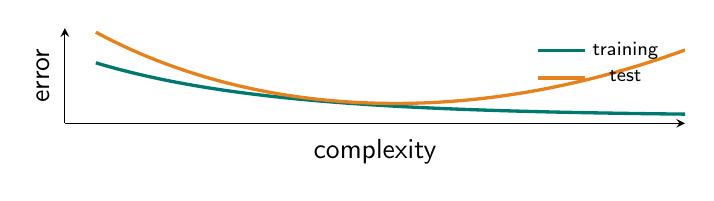
\begin{tikzpicture}
\begin{axis}[
  width=0.78\linewidth,height=0.23\linewidth,
  xmin=0,xmax=10,ymin=0,ymax=1.05,
  axis lines=left,
  xlabel={complexity}, ylabel={error},
  xtick=\empty, ytick=\empty,
  legend style={draw=none,fill=none,font=\scriptsize,at={(0.98,0.98)},anchor=north east}
]
\addplot[very thick,posterGreen,domain=0.5:10,samples=80] {0.70*exp(-0.35*x)+0.08};
\addlegendentry{training}
\addplot[very thick,posterOrange,domain=0.5:10,samples=80] {0.18+0.40*exp(-0.45*x)+0.025*(x-5)^2};
\addlegendentry{test}
\end{axis}
\end{tikzpicture}
\end{center}

\miniheadline{Message.} A class that is too flexible can fit training data without generalising.
}

\block{2. Rademacher Complexity: Can the Class Fit Noise?}{
Let $\epsilon_i\in\{-1,+1\}$ be independent random signs. For real-valued $h\in\Hc$,
\[
\Rad_m(\Hc)=\mathbb{E}_{S,\epsilon}\left[\sup_{h\in\Hc}\frac{1}{m}\sum_{i=1}^{m}\epsilon_i h(z_i)\right].
\]

\miniheadline{Intuition.} The supremum is large when some $h$ aligns with pure random noise.

\begin{center}
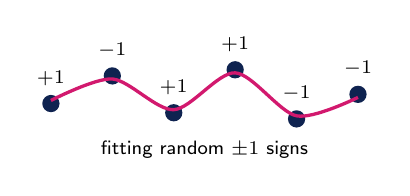
\begin{tikzpicture}[scale=0.78]
  \foreach \x/\y/\lab in {0/0/+1,1/0.45/-1,2/-0.15/+1,3/0.55/+1,4/-0.25/-1,5/0.15/-1}{
    \fill[posterNavy] (\x,\y) circle (4pt);
    \node[above=3pt] at (\x,\y) {\scriptsize $\lab$};
  }
  \draw[posterMagenta,very thick,smooth] plot coordinates {(0,0.05) (1,0.4) (2,-0.1) (3,0.5) (4,-0.2) (5,0.1)};
  \node[align=center] at (2.5,-0.75) {\scriptsize fitting random $\pm1$ signs};
\end{tikzpicture}
\end{center}
}

\block{3. Master Theorem: Complexity Controls the Gap}{
Symmetrisation gives
\[
\mathbb{E}_{S}\left[\sup_{h\in\Hc}\left(\frac1m\sum_{i=1}^m h(z_i)-\mathbb{E}[h(z)]\right)\right]
\le 2\Rad_m(\Hc).
\]

\miniheadline{Proof idea.}
Introduce an independent ``ghost sample'', replace the population expectation by its empirical average, then use random signs to symmetrise the two samples.

\smallbox{Bound $\Rad_m(\Hc)$ $\Rightarrow$ bound generalisation.}
}

\block{4. From Functions to Label Vectors}{
For $\F\subseteq\{\pm1\}^{\X}$ and fixed points $x_1,\ldots,x_m$,
\[
\F|_{x_1^m}
=
\{(f(x_1),\ldots,f(x_m)):f\in\F\}
\subseteq\{\pm1\}^{m}.
\]

\miniheadline{Key idea.}
$|\F|_{x_1^m}|$ counts how many different labelings the class can produce on this dataset.

\vspace{-0.6em}
\begin{center}
Multiple functions can produce the same label vector on a fixed dataset.
\end{center}
\vspace{-0.6em}
}


% COLUMN 2
\column{0.333}

\block{5. Growth Function: Worst-Case Number of Labelings}{
The growth function is
\[
\boxed{
\Pi_{\F}(m)
=
\max_{x_1,\ldots,x_m\in\X}
\left|\F|_{x_1^m}\right|
}
\]

It asks: what is the largest number of distinct binary labelings the class can realise on any $m$ points?

\[
\Pi_{\F}(m)\le 2^m.
\]

\vspace{-0.6em}
\begin{center}
For $m=2$, there are at most $2^2=4$ possible labelings.
\end{center}
\vspace{-0.6em}
}

\block{6. Massart's Lemma: Finite Vectors Bound Rademacher Complexity}{
For finite $A\subset\mathbb{R}^m$ with $r=\sup_{a\in A}\|a\|_2$,
\[
\mathbb{E}_{\epsilon}\left[\sup_{a\in A}\frac1m\sum_{i=1}^m\epsilon_i a_i\right]
\le
\frac{r\sqrt{2\ln |A|}}{m}.
\]

Apply to $A=\F|_{x_1^m}$. Since each binary label vector has $r=\sqrt m$,
\[
\boxed{
\Rad_m(\F)\le\sqrt{\frac{2\ln \Pi_{\F}(m)}{m}}.
}
\]

\begin{center}
Rademacher complexity is controlled by the growth function    
\end{center}

}

\block{7. Why the Trivial Bound Fails}{
Using only $\Pi_\F(m)\le 2^m$ gives
\[
\Rad_m(\F)
\le
\sqrt{\frac{2\ln(2^m)}{m}}
=
\sqrt{2\ln 2}.
\]
This constant does not vanish as $m\to\infty$, so it cannot prove that more data improves generalisation.

\begin{center}
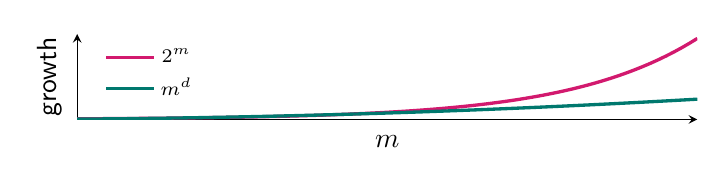
\begin{tikzpicture}
\begin{axis}[
  width=0.78\linewidth,height=0.22\linewidth,
  xmin=1,xmax=8,ymin=0,ymax=270,
  axis lines=left,
  xlabel={$m$}, ylabel={growth},
  xtick=\empty, ytick=\empty,
  legend style={draw=none,fill=none,font=\scriptsize,at={(0.03,0.97)},anchor=north west}
]
\addplot[very thick,posterMagenta,domain=1:8,samples=80] {2^x};
\addlegendentry{$2^m$}
\addplot[very thick,posterGreen,domain=1:8,samples=80] {x^2};
\addlegendentry{$m^d$}
\end{axis}
\end{tikzpicture}
\end{center}
}


% COLUMN 3
\column{0.334}

\block{8. VC Dimension: Where Full Flexibility Stops}{
A set $\{x_1,\ldots,x_m\}$ is \textbf{shattered} by $\F$ if every binary labeling can be realised:
\[
\F|_{x_1^m}=\{\pm1\}^m.
\]

The \textbf{VC dimension} is
\[
\boxed{\mathrm{VCdim}(\F)=\max\{m:\Pi_\F(m)=2^m\}.}
\]

\begin{center}
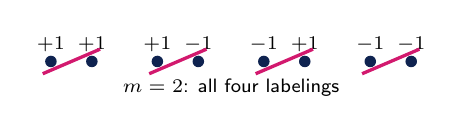
\begin{tikzpicture}[scale=0.52]
  \begin{scope}[xshift=0cm]
    \fill[posterNavy] (0,0) circle (4pt); \fill[posterNavy] (1,0) circle (4pt);
    \node[above] at (0,0) {\scriptsize $+1$}; \node[above] at (1,0) {\scriptsize $+1$};
    \draw[posterMagenta,very thick] (-0.2,-0.3)--(1.2,0.3);
  \end{scope}
  \begin{scope}[xshift=2.6cm]
    \fill[posterNavy] (0,0) circle (4pt); \fill[posterNavy] (1,0) circle (4pt);
    \node[above] at (0,0) {\scriptsize $+1$}; \node[above] at (1,0) {\scriptsize $-1$};
    \draw[posterMagenta,very thick] (-0.2,-0.3)--(1.2,0.3);
  \end{scope}
  \begin{scope}[xshift=5.2cm]
    \fill[posterNavy] (0,0) circle (4pt); \fill[posterNavy] (1,0) circle (4pt);
    \node[above] at (0,0) {\scriptsize $-1$}; \node[above] at (1,0) {\scriptsize $+1$};
    \draw[posterMagenta,very thick] (-0.2,-0.3)--(1.2,0.3);
  \end{scope}
  \begin{scope}[xshift=7.8cm]
    \fill[posterNavy] (0,0) circle (4pt); \fill[posterNavy] (1,0) circle (4pt);
    \node[above] at (0,0) {\scriptsize $-1$}; \node[above] at (1,0) {\scriptsize $-1$};
    \draw[posterMagenta,very thick] (-0.2,-0.3)--(1.2,0.3);
  \end{scope}
  \node at (4.4,-0.65) {\scriptsize $m=2$: all four labelings};
\end{tikzpicture}
\end{center}

\begin{center}
\renewcommand{\arraystretch}{1.05}
\begin{tabular}{lc}
\toprule
Class $\F$ & VCdim$(\F)$ \\
\midrule
Intervals on $\mathbb{R}$ & $2$ \\
Rectangles in $\mathbb{R}^2$ & $4$ \\
Halfspaces in $\mathbb{R}^d$ & $d+1$ \\
Convex polygons in $\mathbb{R}^2$ & $\infty$ \\
\bottomrule
\end{tabular}
\end{center}
}

\block{9. Sauer's Lemma: VC Dimension Controls Growth}{
If $\mathrm{VCdim}(\F)=d$, then
\[
\boxed{
\Pi_{\F}(m)
\le
\sum_{i=0}^{d}\binom{m}{i}.
}
\]

For $m\ge d$,
\[
\boxed{
\Pi_{\F}(m)
\le
\left(\frac{em}{d}\right)^d.
}
\]

\miniheadline{Meaning.} After the class stops shattering beyond $d$ points, growth is polynomial instead of exponential:
\[
2^m \quad \text{becomes roughly} \quad m^d.
\]
}

\block{10. Final Chain: VC Dimension Upper-Bounds Rademacher Complexity}{
For $m\ge d$,
\[
\Rad_m(\F)
\le
\sqrt{\frac{2\ln\Pi_\F(m)}{m}}
\le
\boxed{\sqrt{\frac{2d\ln(em/d)}{m}}}.
\]

Therefore,
\[
\boxed{
\mathbb{E}_{S}\left[\sup_{f\in\F}\bigl(\widehat R(f)-R(f)\bigr)\right]
\lesssim
\sqrt{\frac{d\ln(em/d)}{m}}.
}
\]
}

\block{11. Takeaway and References}{
\begin{center}
\Large\textbf{A class generalises when it cannot realise too many labelings relative to the amount of data.}
\end{center}

\vspace{0.2em}
\begin{center}

\begin{tikzpicture}[node distance=0.55cm,scale=0.78,transform shape]
  \node[draw,rounded corners,fill=posterTealLight,minimum width=3.2cm] (gap) {gap};
  \node[draw,rounded corners,fill=posterTealLight,minimum width=3.2cm,right=of gap] (rad) {Rademacher};
  \node[draw,rounded corners,fill=posterTealLight,minimum width=3.2cm,right=of rad] (growth) {growth};
  \node[draw,rounded corners,fill=posterTealLight,minimum width=3.2cm,right=of growth] (vc) {VC dim};
  \draw[-{Latex[length=3mm]},thick] (gap)--(rad);
  \draw[-{Latex[length=3mm]},thick] (rad)--(growth);
  \draw[-{Latex[length=3mm]},thick] (growth)--(vc);
\end{tikzpicture}
\end{center}

\small
\textbf{References:} COMP34312 course notes; Kakade \& Tewari Lectures 10--11; Vapnik--Chervonenkis (1971); Sauer (1972).
}

\end{columns}
\end{document}